\chapter{Courbes classés} \label{chap:courbeClasses}

\section{Introduction de l'exemple}
Nous avons l'exemple suivant (\texttt{fichier : 0\_4\_1\_courbe\_debits\_classes.xlsx}): \\
\fbox{ %fbox est utilisé pour voir les bords de la minipage
    \begin{minipage}[l]{17cm}
        On dispose des débits journaliers du bassin \og le Parimbot \fg{} à la station d'Ecublens (FR, CH). \\

        \begin{tabular}{|l|r|}
            \hline
            \textbf{Date} & \textbf{Débit moyen journalier} [L/s] \\
            \hline
            01.01.1979    & 361.073                               \\
            02.01.1979    & 180.573                               \\
            \dots         & \dots                                 \\
            30.12.1993    & 268.555                               \\
            31.12.1993    & 2166.966                              \\
            \hline
        \end{tabular}
        \\ \\
        \textbf{Question 1 :} Construire la courbe des débits classés ; pour la méthode globale et la période 1979 - 1993. \\
        \textbf{Question 2 :} Calculer les débits caractéristiques d'étiage (DCE, DC10, Q347) à partir de la courbe. \\
        \textbf{Question 3 :} Déterminer les possibilités d'accorder une concession de pompage de 30 L/s en se basant sur le calcul du débit résiduel minimal. \\
        \textbf{Question 4 :} Construire la courbe des débits classés par la méthode de la moyenne des courbes annuelles. Intérêt de cette méthode ?
    \end{minipage}
}

\section{Question 1}
\subsection{Méthode à appliquer}
\begin{itemize}
    \item La courbe des débits classés : nombre de jours (ou pourcentage du temps) durant lesquels la valeur du débit moyen journalier $Q$ a été atteinte ou dépassés
    \item On fixe : \\
    \begin{itemize}
        \item $n$ : nombre d'années d'étude
        \item $N$ : nombre de débits 
        \item $x$ : correspond au nombre de jours pendant les $n$ années où le débit $Q$ a été dépassé
        \item La fréquence est $f_i = \cfrac{x}{\cfrac{N}{365}}$
    \end{itemize}
\end{itemize}

\subsection{Démarche et résultats}
\begin{enumerate}
    \item Nombre de données de débits moyens journaliers $N=5479$, $n=15$ ;
    \item Classer les données par ordre décroissant et donner un rang $r$ à chaque valeur
    \item Calcul de la fréquence annuelle pour chaque débit $Q$ : $f = \cfrac{r}{N}\cdot 365$
    \item Représentation graphique
\end{enumerate}

\subsection{Solution}
\begin{tabular}{|ccc|}
    \hline
    \textbf{Rang} & \textbf{Prob.} & \textbf{Q classés} \\
    1             & 0.1           & 7237.75             \\
    2             & 0.1           & 6323.113            \\
    \dots         & \dots         & \dots               \\
    364.9         & 5478          & 0.0                 \\
    635           & 5479          & 0.0                 \\
    \hline
\end{tabular}

\begin{figure}[H]
    \centering
    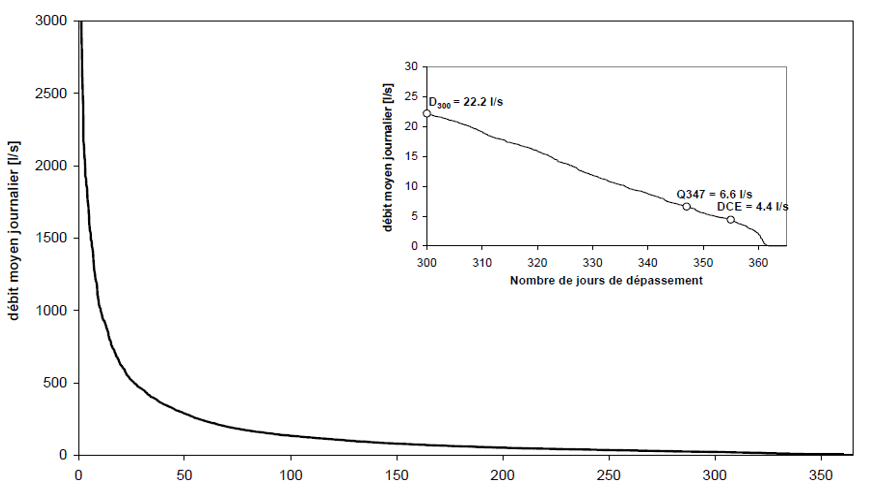
\includegraphics[width=15cm]{courbeClasses_graph.png}
    \caption{Courbe des débits classés (méthode globale) et débits caractéristiques d'étiage}
\end{figure}

\section{Question 2}
\subsection{Méthode à appliquer}
Lire les débits caractéristiques d'étiage à partir de la courbe des débits classés

\subsection{Résultats}
\begin{tabular}{|ccc|}
    \hline
    \textbf{Rang} & \textbf{Prob.} & \textbf{Q classés} \\
    \hline
    300.0         & 4503           & 22.1746             \\
    300.0         & 4504           & 22.1694             \\
    \hline
    DC10 = $\text{Q300}_\text{moyen}$ &   & 22.1720      \\
    \hline
    347.0         & 5209           & 6.5937              \\
    \hline
    355.0         & 5329           & 4.3681              \\
    \hline
\end{tabular}

\section{Question 3}
Selon la figure \ref{fig:loiQ347} ; le débit minimal à garantir est de 50 L/s. 
Cela signifie qu'après pompage, le débit résiduel (débit restant dans le cours d'eau) ne doit pas être inférieur à cette valeur seuil.
Le captage ne pourra se faire que si le débit en amont de la prise d'eau est supérieur strictement à 80 l/s.

\section{Question 4}
On établit pour chaque année la courbe des débits classés, et on peut ensuite faire une moyenne arithmétique de toutes les années d'études.
Cette méthode permet de visualiser les incertitudes sur les débits caractéristiques d'étiage.

\begin{figure}[H]
    \centering
    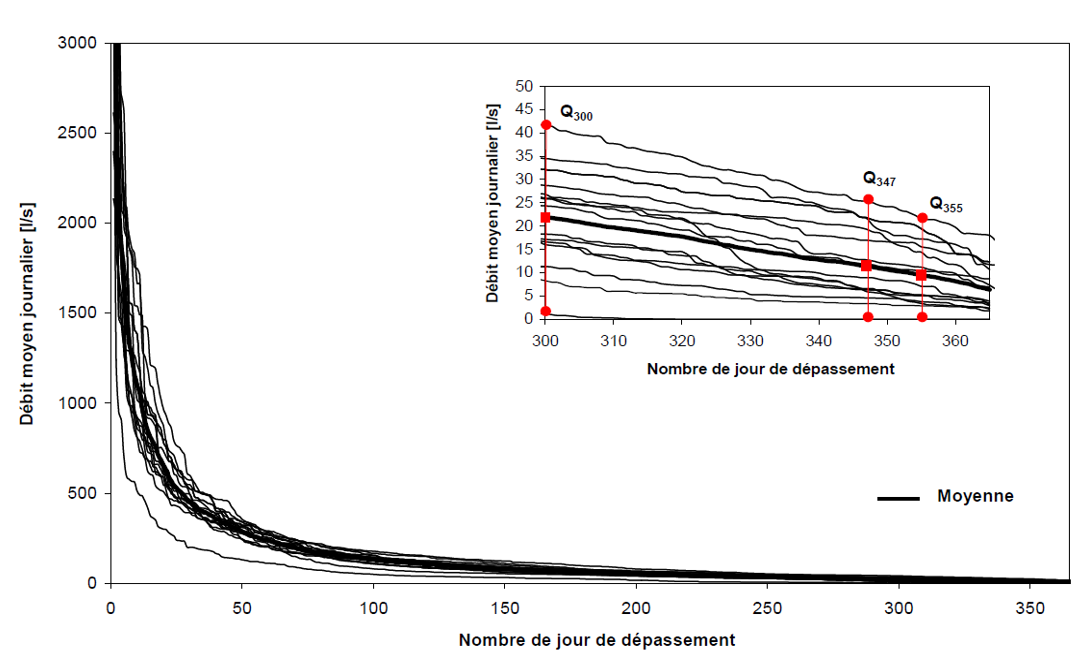
\includegraphics[width=15cm]{courbeClasses_graph2.png}
    \caption{Courbe des débits classés (méthode de la moyenne des courbes annuelles) et débits caractéristiques d'étiage}
\end{figure}
